\documentclass{minimal}
\usepackage{tikz}

\begin{document}
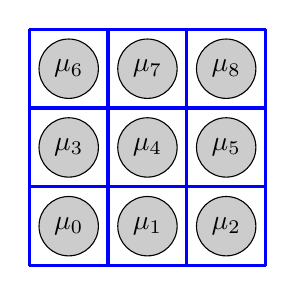
\begin{tikzpicture}[darkstyle/.style={circle,draw,fill=gray!40,minimum size=20}]

    \newcommand*{\cellsize}{1}%
    \newcommand*{\numcells}{3}%

    \draw [step=\cellsize, blue, very thick] (0,0) grid ({\cellsize*\numcells},{\cellsize*\numcells});


  \foreach \x in {0,...,2}
    \foreach \y in {0,...,2}
    %    {\pgfmathtruncatemacro{\label}{\x - 5 *  \y +21}
       {\pgfmathtruncatemacro{\label}{3 * \y + \x}
       \node [darkstyle]  (\x\y) at ({\x + \cellsize / 2},{\y + \cellsize / 2}) {$\mu_{\label}$};}

%   \foreach \x in {0,...,\numcells}
%     \foreach \y [count=\yi] in {0,...,\numcells}
%       \draw (\x\y)--(\x\yi) (\y\x)--(\yi\x) ;

\end{tikzpicture}
\end{document}
